\nexthint{Example - Slide stm. abs.}
\begin{frame}{Object equality}
REFINITY lacked rules for object equality over multiple modalities:
\begin{itemize}
\item can verify \refa{Slide Statement} with abstract statements
\end{itemize}
\end{frame}

\nexthint{Object equality II}
\begin{frame}\vspace*{-5mm}
\begin{center}
  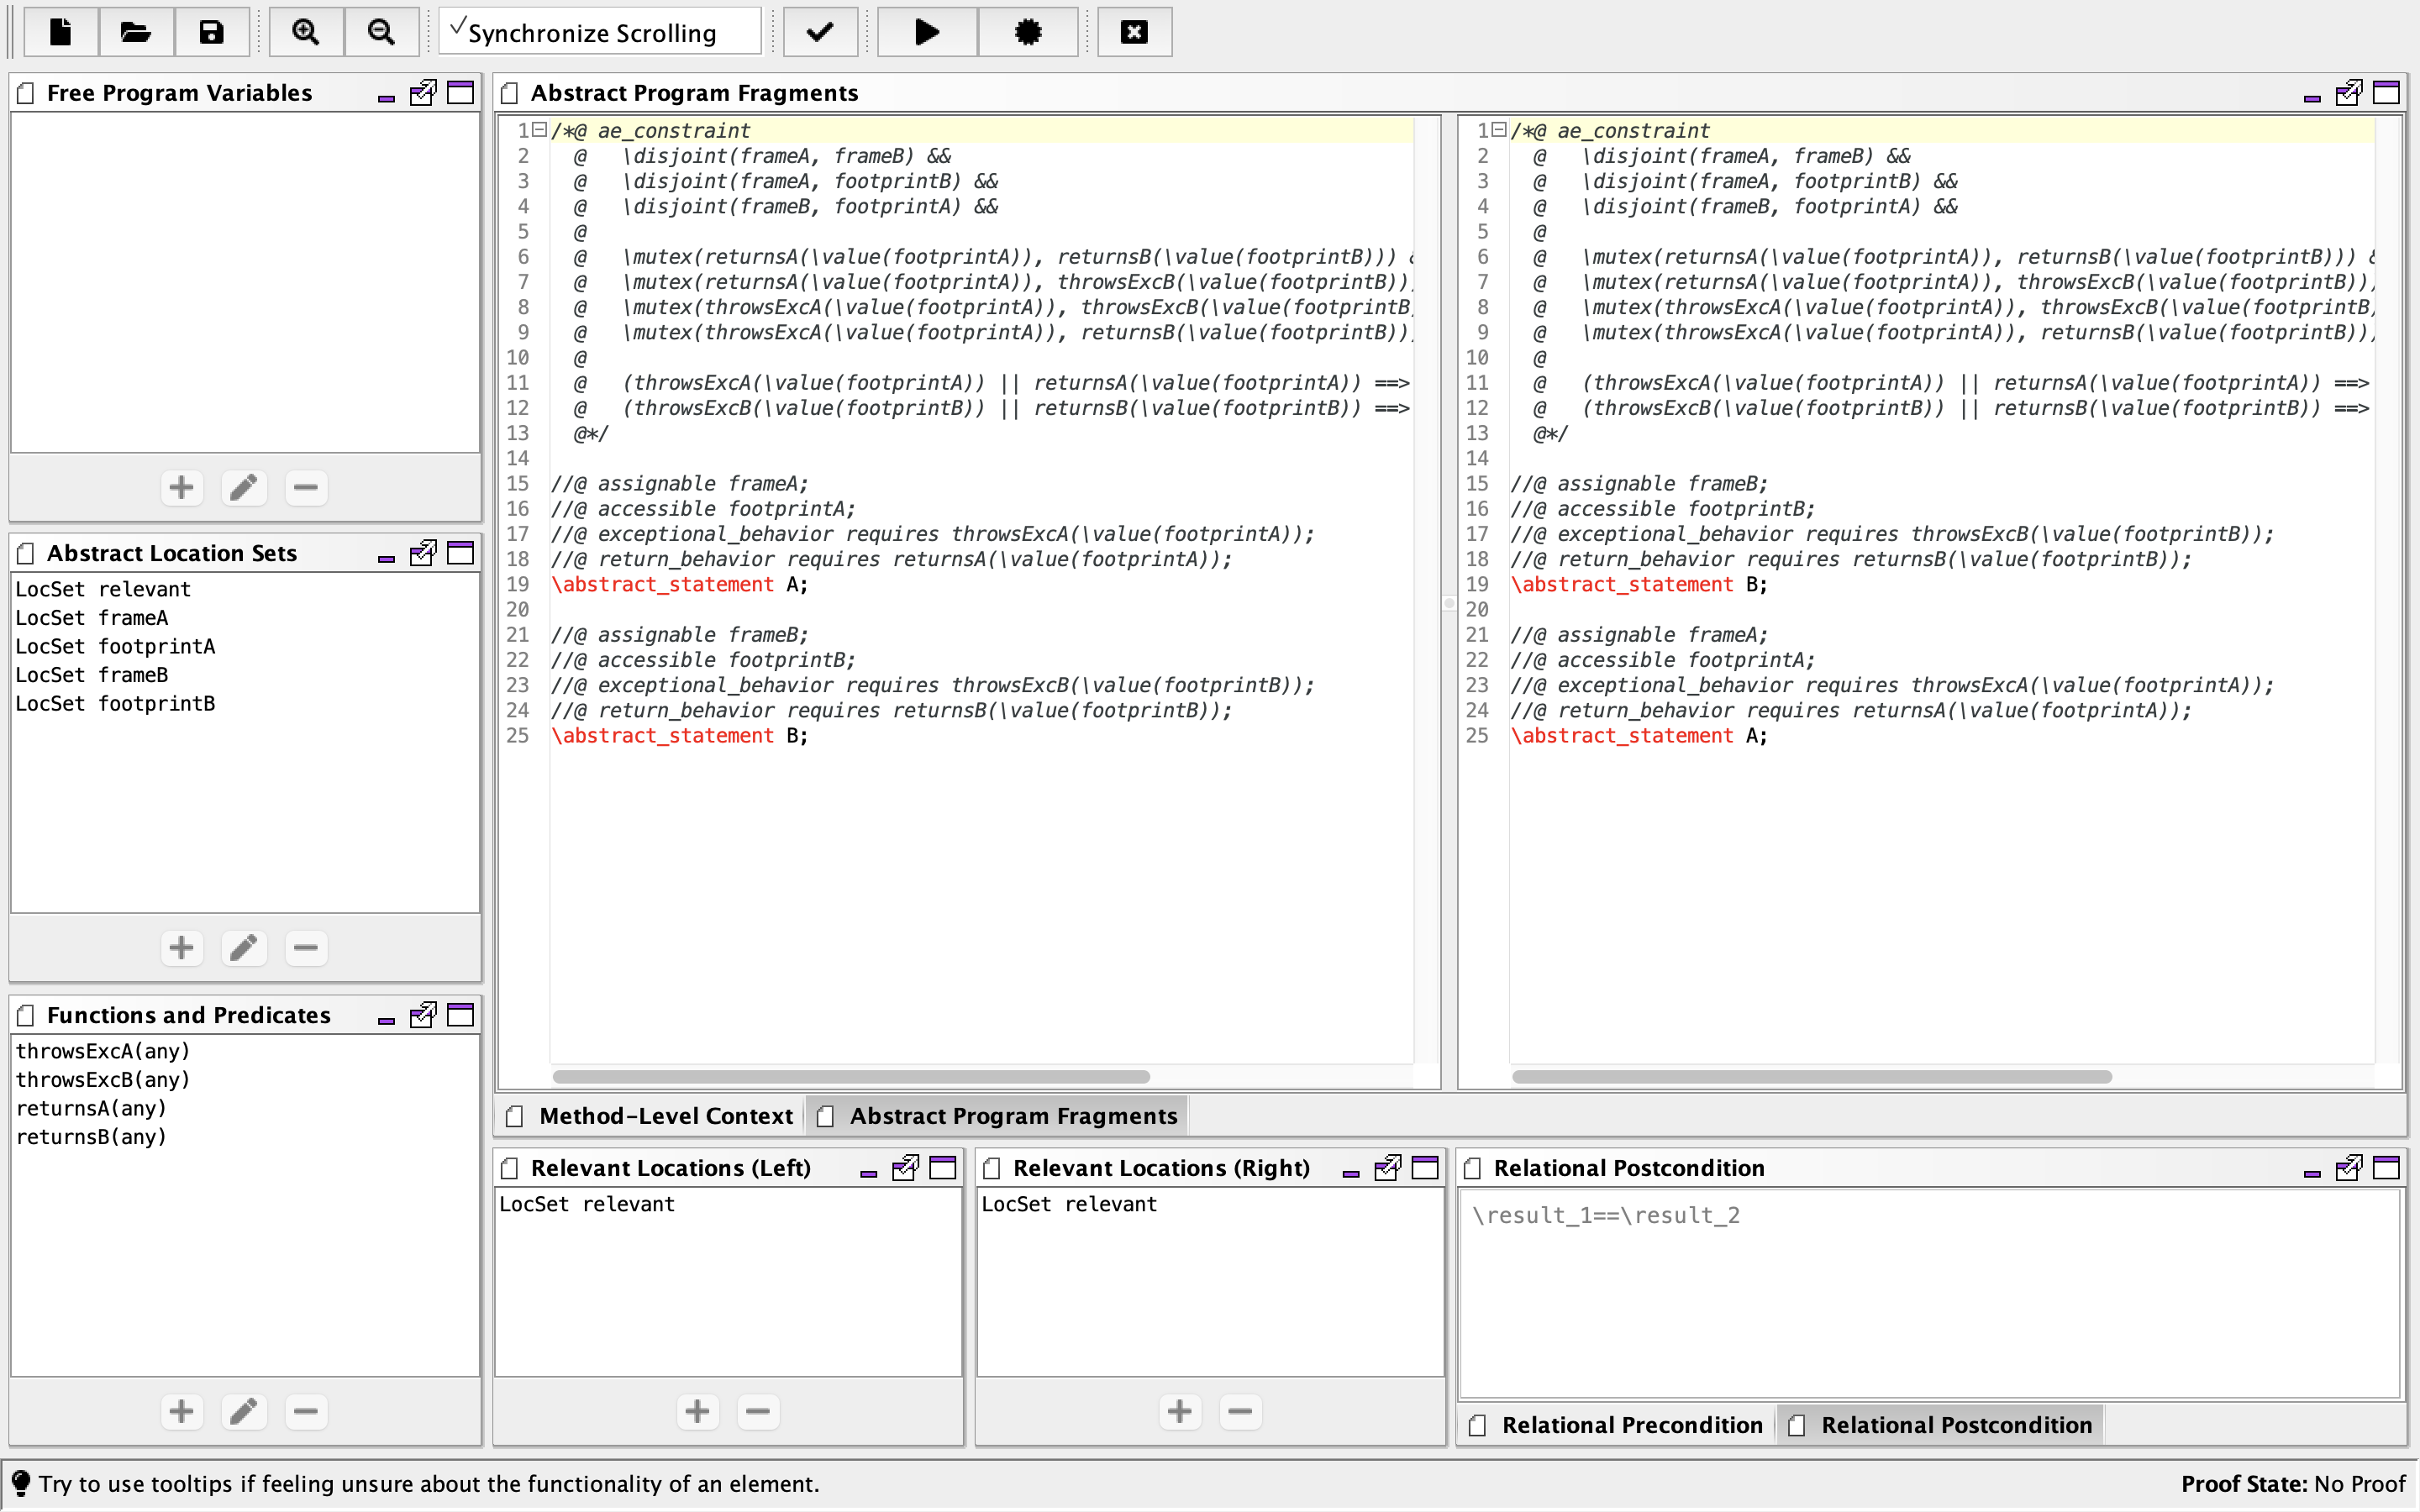
\includegraphics[scale=.25]{screenshots/SlideAbstract}
\end{center}
\end{frame}

\nexthint{Example - Slide stm. conc.}
\begin{frame}{Object equality}
REFINITY lacked rules for object equality over multiple modalities:
\begin{itemize}
\item can verify Slide Statement with abstract statements
\item can't verify Slide Statement with statements involving concrete objects
\end{itemize}
\end{frame}

\nexthint{Why?}
\begin{frame}\vspace*{-5mm}
\begin{center}
  \includegraphics[scale=.25]{screenshots/Slide}
\end{center}
\end{frame}

\nexthint{Adding taclets and rules}
\begin{frame}{REFINITY Internals}
  Core issue:
  \begin{itemize}
    \item Objects are placed in a symbolic heap during SE
    \item Before and After program executed in same proof
    \end{itemize}

\medskip    
Not sufficient for two new objects to be equal:
  \begin{itemize}
    \item the allocation must, additionally, be deterministic
  \end{itemize}
\end{frame}


%taclets
%They contain the declarative, logical content of the rule schemata, but also pragmatic information:
%in which context and when a rule should be applied by an automated reasoning strategy and how it is to be presented to the user.
%At the core of the KeY system is an efficient interpreter that applies taclets to goal sequents and thereby constructs proof trees.
\nexthint{Definition 1}
\begin{frame}{Adding rules required for object equality}
  Schematic sequent rules in KeY are specified as \textit{taclets}:
  \begin{itemize}
  \item we add rules to make objects indistinguishable under under certain conditions
  \end{itemize}
\end{frame}

\nexthint{Definition 2}
% \begin{frame}
%   \begin{center}
%   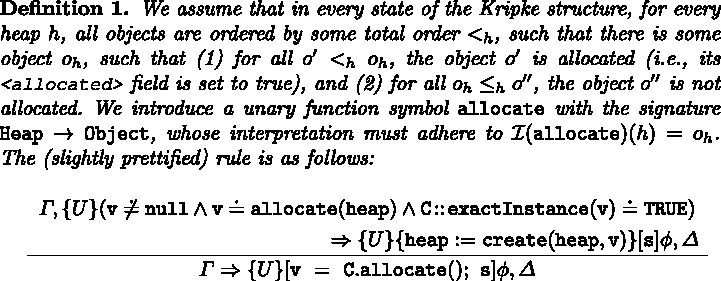
\includegraphics{imported/Definition1}
%   \end{center}
% \end{frame}

\nexthint{Postcondition simplification}
\begin{frame}{New \textit{taclet} for object creation}
  \begin{center}
  \includegraphics[width=\linewidth]{imported/Definition2}
  \end{center}
\end{frame}

\nexthint{Example - Hide Delegate (default postcondition)}
\begin{frame}{Postcondition simplification}
In \refa{Hide Delegate} exception objects now equivalent
\begin{itemize}
  \item we need no special postcondition to handle exceptions\ldots
    \item \ldots although we should because in practice exceptions
      capture state! {\small (Not \emph{our} problem, though \emoji{upside-down-face})}
  \end{itemize}
\end{frame}

\nexthint{Future challenges}
\begin{frame}\vspace*{-5mm}
  \begin{center}
  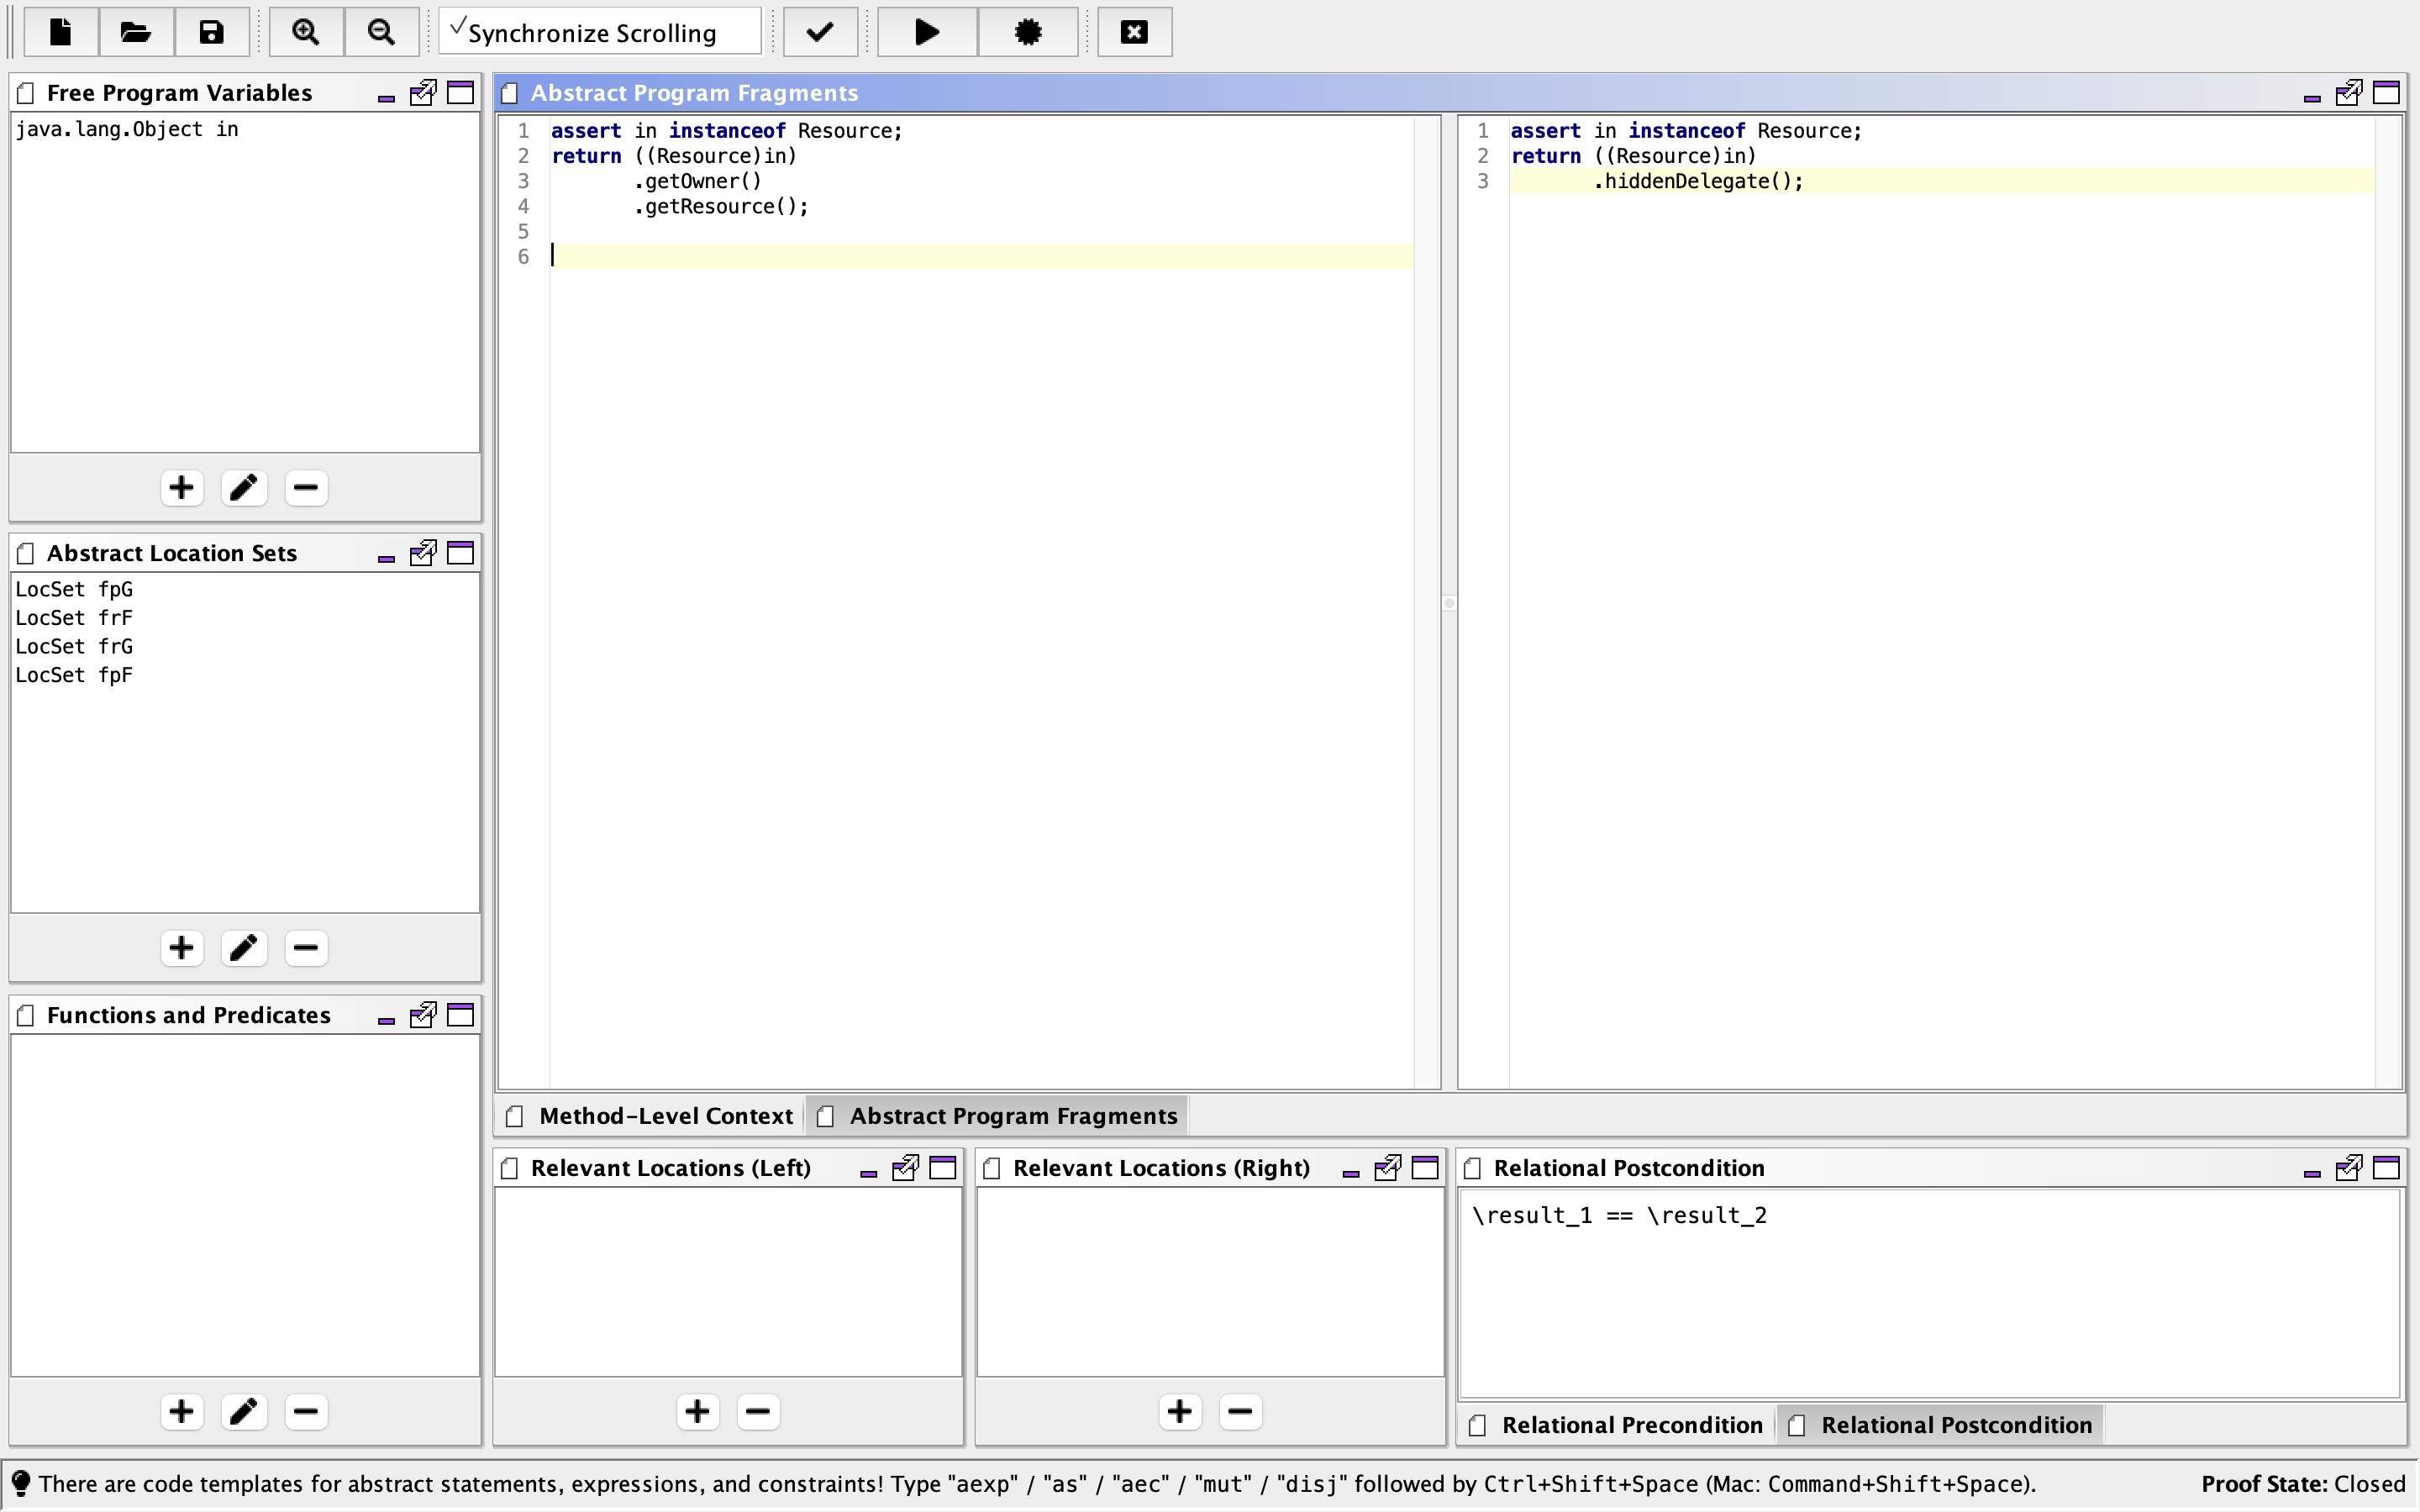
\includegraphics[scale=0.25]{screenshots/HideDelegateDefaultPostcondition}
  \end{center}
\end{frame}

